\subsection{Cahier des charges}

Dans le but de développer la bibliothèque nous avons établi un cahier des charges encadrant les trois ensembles de fonctionnalités qui la constitue:
\begin{itemize}
\item Pré-traitement des images
\item Detection des évolutions d'un dessin
\item Reconnaissance des formes dessinées
\end{itemize}

\subsubsection{Pré-traitement}

Tout traitement sur une image nécesite d'effectuer un certain nombre de pré-traitement afin d'en améliorer la qualité. Cet étape à pour but de favoriser l'obtention de bon résultats lors de la phase de traitement.

La bibliothèque devra permettre d'appliquer aisément un certain nombre de filtre, notament:

\begin{description}
\item[Filtre morphologique] Optimisation de la detection de zones avec des formes
\item[Binarisation] Permettre de trouver les différences qui existent entre deux images
\item[Correction de couleur] Balance des blancs, permet d'annuler la coloration globale de l'image dépendante de l'éclairage de la scène (lumière du jour ou lumière artificielle)
\item[Filtrage par couleur] Recupérer uniquement les formes dessiné avec une couleur précise.
\end{description}


\subsubsection{Detection des évolutions d'un dessin}



\subsubsection{Reconnaissance des formes dessinées}
\begin{itemize}
\item Mise en correspondance à partir d’1 image de référence (forme simples)
\item Feature detection (SIFT FAST MSER) (forme complexe)
\item Reconnaissance à partir d’un BDD => cascade / SVM classifier (objets simples dans une image complexe)
\end{itemize}
optimisation 10 fps (utilisation des nouveautés dans l’image)


\subsection{Planning}

\begin{center}
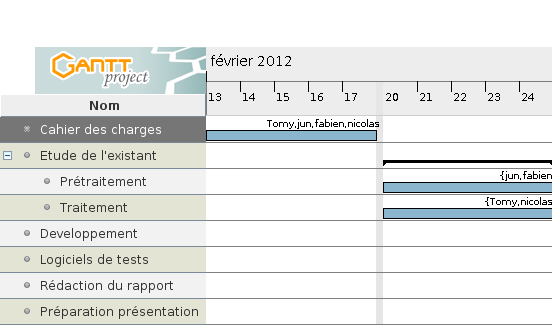
\includegraphics[width=\textwidth]{gantt1.png}
\captionof{figure}{Planning taches préparatoire}
\end{center}
\begin{center}
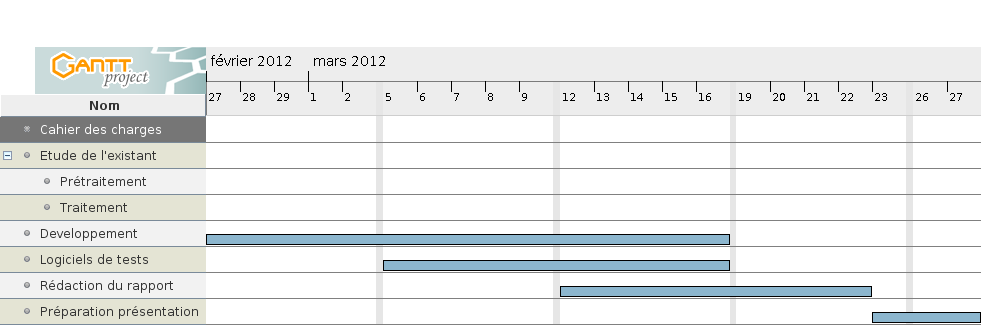
\includegraphics[width=\textwidth]{gantt2.png}
\captionof{figure}{Planning de dévelopement et de fin de projet}
\end{center}